\section{Fases de um compilador}

\begin{frame}[fragile]{As fases de um compilador}

    \begin{itemize}
        \item Conceitualmente, o compilador opera em fases
       %\pause

        \item Cada fase manipula o programa fonte e entrega o resultado para a próxima fase
       %\pause

        \item Na prática, algumas fases podem ser agrupadas, e a representação intermediária entre elas pode ser não se construída explicitamente
       %\pause

        \item As primeiras fases estão relacionadas à análise do programa fonte, as últimas estão relacionadas à síntese (construção do programa alvo)
       %\pause

        \item Duas atividades interagem com todas as fases: a gerência da tabela de símbolos e o tratamento de erros
    \end{itemize}

\end{frame}

\begin{frame}[fragile]{Representação típica das fases de um compilador}

    \begin{figure}
        \centering

        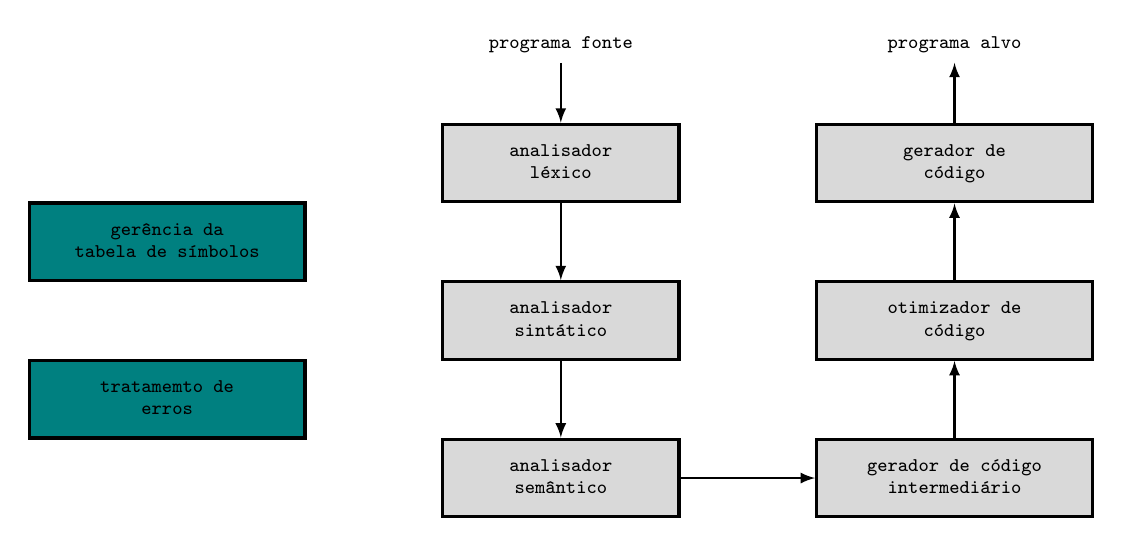
\begin{tikzpicture} 
            \node (A) at (5, 6.5) { \scriptsize \texttt{programa fonte} };
            \node[draw,very thick,fill=gray!30,minimum width=3cm,inner sep=6pt] (B) at (5, 5) { \scriptsize \begin{tabular}{c}\texttt{analisador}\\\texttt{léxico}\end{tabular} };
            \node[draw,very thick,fill=gray!30,minimum width=3cm,inner sep=6pt] (C) at (5, 3) { \scriptsize \begin{tabular}{c}\texttt{analisador}\\\texttt{sintático}\end{tabular} };
            \node[draw,very thick,fill=gray!30,minimum width=3cm,inner sep=6pt] (D) at (5, 1) { \scriptsize \begin{tabular}{c}\texttt{analisador}\\\texttt{semântico}\end{tabular} };
            \node[draw,very thick,fill=gray!30,minimum width=3.5cm,inner sep=6pt] (E) at (10, 1) { \scriptsize \begin{tabular}{c}\texttt{gerador de código}\\\texttt{intermediário}\end{tabular} };
            \node[draw,very thick,fill=gray!30,minimum width=3.5cm,inner sep=6pt] (F) at (10, 3) { \scriptsize \begin{tabular}{c}\texttt{otimizador de}\\\texttt{código}\end{tabular} };
            \node[draw,very thick,fill=gray!30,minimum width=3.5cm,inner sep=6pt] (G) at (10, 5) { \scriptsize \begin{tabular}{c}\texttt{gerador de}\\\texttt{código}\end{tabular} };
            \node (H) at (10, 6.5) { \scriptsize \texttt{programa alvo} };

            \node[draw,very thick,fill=blue!50!green,minimum width=3.5cm,inner sep=6pt] (I) at (0, 4) { \scriptsize \begin{tabular}{c}\texttt{gerência da}\\\texttt{tabela de símbolos}\end{tabular} };
            \node[draw,very thick,fill=blue!50!green,minimum width=3.5cm,inner sep=6pt] (J) at (0, 2) { \scriptsize \begin{tabular}{c}\texttt{tratamemto de}\\\texttt{erros}\end{tabular} };

            \draw[thick,-latex] (A) to (B);
            \draw[thick,-latex] (B) to (C);
            \draw[thick,-latex] (C) to (D);
            \draw[thick,-latex] (D) to (E);
            \draw[thick,-latex] (E) to (F);
            \draw[thick,-latex] (F) to (G);
            \draw[thick,-latex] (G) to (H);

        \end{tikzpicture} 
    \end{figure}

\end{frame}

\begin{frame}[fragile]{Gerenciamento da tabela de símbolos}

    \begin{itemize}
        \item Esta atividade registra os identificadores do programa alvo e identifica seus diversos atributos
       %\pause

        \item Exemplos de possíveis atributos de um identificador: nome, tipo, memória e escopo
       %\pause

        \item Caso o identificador se refira a um procedimento, dentre seus atributos devem constar a quantidade de seus parâmetros e respectivos tipos, modo 
            de passagem (cópia ou referência) e o tipo do retorno, se houver
       %\pause

        \item Os identificadores e seus respectivos atributos são armazenados em uma estrutura denominada tabela de símbolos
    \end{itemize}

\end{frame}

\begin{frame}[fragile]{Tratamento de erros}

    \begin{itemize}
        \item A cada fase da compilação podem acontecer um ou mais erros
       %\pause

        \item Após a identificação do erro, o compilador deve tratá-lo de alguma maneira e, se possível, continuar o processo em busca de outros erros
       %\pause

        \item Abortar a compilação logo no primeiro erro pode diminuir a utilidade do compilador (por exemplo, o prosseguimento da compilação após um erro
            léxico pode ajudar na geração de uma sugestão de correção para o erro)
       %\pause

        \item As análises sintática e semântica podem identificar uma parcela considerável dos erros no programa fonte
    \end{itemize}

\end{frame}

\begin{frame}[fragile]{Exemplo da parte da análise do programa fonte}

    \begin{figure}
        \centering 

        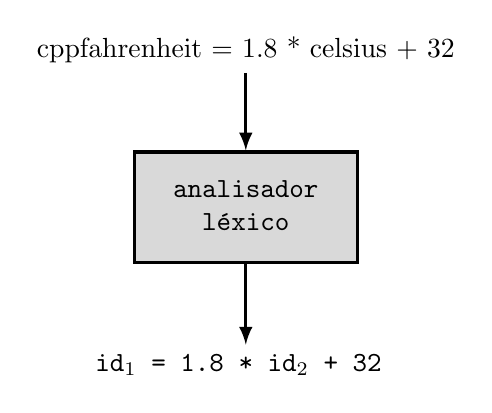
\begin{tikzpicture}
            \node (A) at (6, 6) { \code{cpp}{fahrenheit = 1.8 * celsius + 32} };
            \node[draw,very thick,fill=gray!30,inner sep=8pt] (B) at (6, 4) { \begin{tabular}{c}\texttt{analisador}\\ \texttt{léxico}\end{tabular} };
            \node (C) at (6, 2) { \texttt{\textbf{id}$_1$ = 1.8 * \textbf{id}$_2$ + 32 } };

            \draw[very thick,-latex] (A) to (B);
            \draw[very thick,-latex] (B) to (C);
        \end{tikzpicture}

        \caption{Análise léxica do enunciado \code{cpp}{fahrenheit = 1.8 * celsius + 32} }
    \end{figure}

\end{frame}

\begin{frame}[fragile]{Exemplo da parte da análise do programa fonte}

    \begin{figure}
        \centering 

        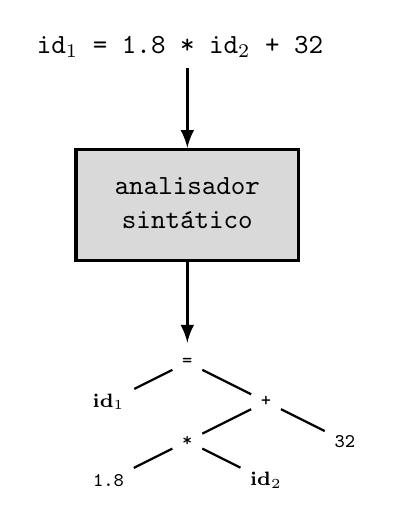
\begin{tikzpicture}
            \node (X) at (6, 6) { \texttt{\textbf{id}$_1$ = 1.8 * \textbf{id}$_2$ + 32 } };
            \node[draw,very thick,fill=gray!30,inner sep=8pt] (Y) at (6, 4) { \begin{tabular}{c}\texttt{analisador}\\ \texttt{sintático}\end{tabular} };

            \node (A) at (5, 1.5) { \scriptsize \textbf{id}$_1$ };
            \node (B) at (6, 2) { \scriptsize \texttt{=} };
            \node (C) at (7, 1.5) { \scriptsize \texttt{+} };
            \node (D) at (6, 1) { \scriptsize \texttt{*} };
            \node (E) at (5, 0.5) { \scriptsize \texttt{1.8} };
            \node (F) at (7, 0.5) { \scriptsize \textbf{id}$_2$ };
            \node (G) at (8, 1) { \scriptsize \texttt{32} };

            \draw[thick] (A) to (B);
            \draw[thick] (C) to (B);
            \draw[thick] (C) to (D);
            \draw[thick] (E) to (D);
            \draw[thick] (D) to (F);
            \draw[thick] (C) to (G);
 
            \draw[very thick,-latex] (X) to (Y);
            \draw[very thick,-latex] (Y) to (6, 2.25);
        \end{tikzpicture}

        \caption{Análise sintática}
    \end{figure}

\end{frame}

\begin{frame}[fragile]{Exemplo da parte da análise do programa fonte}

    \begin{figure}
        \centering 

        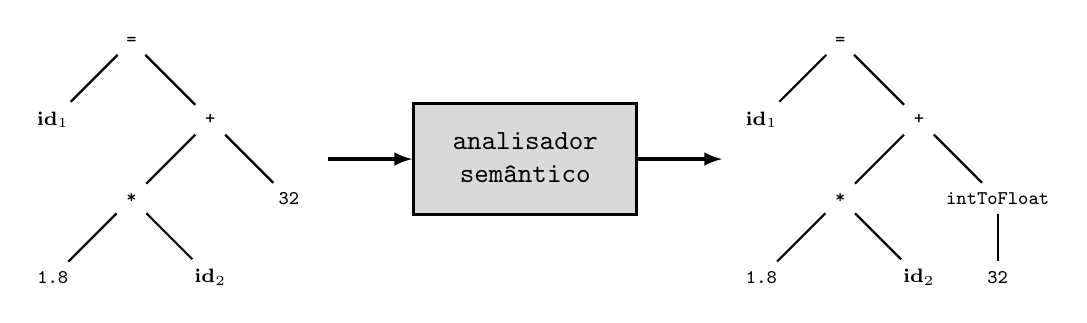
\begin{tikzpicture}
            \node (A1) at (0, 4) { \scriptsize \textbf{id}$_1$ };
            \node (B1) at (1, 5) { \scriptsize \texttt{=} };
            \node (C1) at (2, 4) { \scriptsize \texttt{+} };
            \node (D1) at (1, 3) { \scriptsize \texttt{*} };
            \node (E1) at (0, 2) { \scriptsize \texttt{1.8} };
            \node (F1) at (2, 2) { \scriptsize \textbf{id}$_2$ };
            \node (G1) at (3, 3) { \scriptsize \texttt{32} };

            \draw[thick] (A1) to (B1);
            \draw[thick] (C1) to (B1);
            \draw[thick] (C1) to (D1);
            \draw[thick] (E1) to (D1);
            \draw[thick] (D1) to (F1);
            \draw[thick] (C1) to (G1);
 

            \node[draw,very thick,fill=gray!30,inner sep=8pt] (Y) at (6, 3.5) { \begin{tabular}{c}\texttt{analisador}\\ \texttt{semântico}\end{tabular} };

            \node (A) at (9, 4) { \scriptsize \textbf{id}$_1$ };
            \node (B) at (10, 5) { \scriptsize \texttt{=} };
            \node (C) at (11, 4) { \scriptsize \texttt{+} };
            \node (D) at (10, 3) { \scriptsize \texttt{*} };
            \node (E) at (9, 2) { \scriptsize \texttt{1.8} };
            \node (F) at (11, 2) { \scriptsize \textbf{id}$_2$ };
            \node (G) at (12, 3) { \scriptsize \texttt{intToFloat} };
            \node (H) at (12, 2) { \scriptsize \texttt{32} };

            \draw[thick] (A) to (B);
            \draw[thick] (C) to (B);
            \draw[thick] (C) to (D);
            \draw[thick] (E) to (D);
            \draw[thick] (D) to (F);
            \draw[thick] (C) to (G);
            \draw[thick] (G) to (H);
 
            %\draw[very thick,-latex] (X) to (Y);
            \draw[very thick,-latex] (Y) to (8.5, 3.5);
            \draw[very thick,latex-] (Y) to (3.5, 3.5);
        \end{tikzpicture}

        \caption{Análise semântica}
    \end{figure}

\end{frame}

\begin{frame}[fragile]{Geração de código intermédiario}

    \begin{itemize}
        \item A árvore resultante da análise semântica é transformada pelo compilador em um código intermediário
       %\pause

        \item Esta representação pode ser entendida como um código para uma máquina abstrata
       %\pause

        \item O código intermediário deve ter duas qualidades fundamentais:
       %\pause
        \begin{enumerate}
            \item deve ser fácil de gerar
           %\pause

            \item deve ser fácil de traduzir para o programa alvo
        \end{enumerate}
       %\pause

        \item Uma representação possível é o código de três endereços
       %\pause

        \item Além de computar expressões, esta representação também precisa tratar dos fluxos de controle e das chamadas de procedimentos
    \end{itemize}

\end{frame}

\begin{frame}[fragile]{Exemplo de geração de código intermediário}

    \begin{figure}
        \centering 

        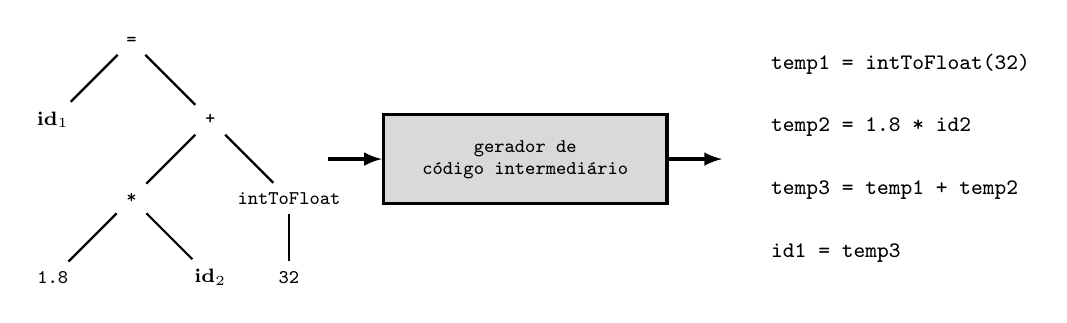
\begin{tikzpicture}

            \node (A) at (0, 4) { \scriptsize \textbf{id}$_1$ };
            \node (B) at (1, 5) { \scriptsize \texttt{=} };
            \node (C) at (2, 4) { \scriptsize \texttt{+} };
            \node (D) at (1, 3) { \scriptsize \texttt{*} };
            \node (E) at (0, 2) { \scriptsize \texttt{1.8} };
            \node (F) at (2, 2) { \scriptsize \textbf{id}$_2$ };
            \node (G) at (3, 3) { \scriptsize \texttt{intToFloat} };
            \node (H) at (3, 2) { \scriptsize \texttt{32} };

            \draw[thick] (A) to (B);
            \draw[thick] (C) to (B);
            \draw[thick] (C) to (D);
            \draw[thick] (E) to (D);
            \draw[thick] (D) to (F);
            \draw[thick] (C) to (G);
            \draw[thick] (G) to (H);
 
            \node[draw,very thick,fill=gray!30,inner sep=8pt] (Y) at (6, 3.5) { \scriptsize \begin{tabular}{c}\texttt{gerador de}\\ \texttt{código intermediário}\end{tabular} };

            \node[anchor=west] at (9, 4.7) { \footnotesize \texttt{temp1 = intToFloat(32)} };
            \node[anchor=west] at (9, 3.9) { \footnotesize \texttt{temp2 = 1.8 * id2} };
            \node[anchor=west] at (9, 3.1) { \footnotesize \texttt{temp3 = temp1 + temp2} };
            \node[anchor=west] at (9, 2.3) { \footnotesize \texttt{id1 = temp3} };

            \draw[very thick,-latex] (Y) to (8.5, 3.5);
            \draw[very thick,latex-] (Y) to (3.5, 3.5);
        \end{tikzpicture}

        \caption{Representação por código de três endereços}
    \end{figure}

\end{frame}

\begin{frame}[fragile]{Otimização do código}

    \begin{itemize}
        \item Esta fase procura formas de melhorar o código intermediário, com o intuito de melhorar a performance do código de máquina do programa alvo
       %\pause

        \item Algumas otimizações são triviais, outras demandam algoritmos sofisticados, impactando no tempo de compilação
       %\pause

        \item As otimizações não devem alterar a semântica do código intermediário
       %\pause

        \item As otimizações podem melhorar, além do tempo de execução, o uso de memória do programa alvo
    \end{itemize}

\end{frame}

\begin{frame}[fragile]{Exemplo de otimização do código intermediário}

    \begin{figure}
        \centering 

        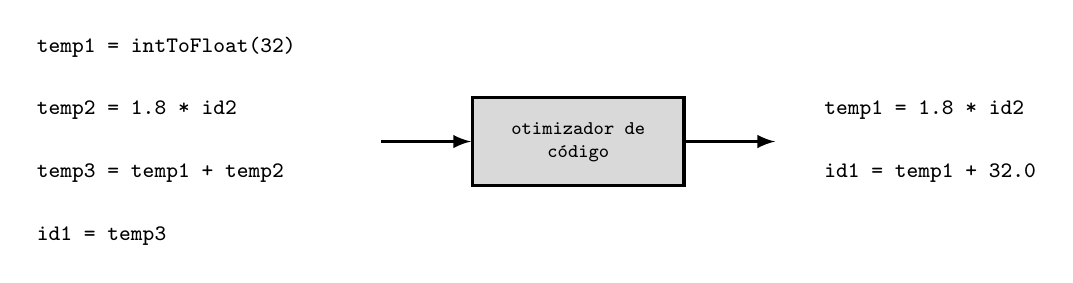
\begin{tikzpicture}

            \node[anchor=west] at (-1, 4.7) { \footnotesize \texttt{temp1 = intToFloat(32)} };
            \node[anchor=west] at (-1, 3.9) { \footnotesize \texttt{temp2 = 1.8 * id2} };
            \node[anchor=west] at (-1, 3.1) { \footnotesize \texttt{temp3 = temp1 + temp2} };
            \node[anchor=west] at (-1, 2.3) { \footnotesize \texttt{id1 = temp3} };

            \node[draw,very thick,fill=gray!30,inner sep=8pt] (Y) at (6, 3.5) { \scriptsize \begin{tabular}{c}\texttt{otimizador de}\\ \texttt{código}\end{tabular} };

            \node[anchor=west] at (9, 3.9) { \footnotesize \texttt{temp1 = 1.8 * id2} };
            \node[anchor=west] at (9, 3.1) { \footnotesize \texttt{id1 = temp1 + 32.0} };

            \draw[very thick,-latex] (Y) to (8.5, 3.5);
            \draw[very thick,latex-] (Y) to (3.5, 3.5);
        \end{tikzpicture}

        \caption{Otimização}
    \end{figure}

\end{frame}

\begin{frame}[fragile]{Geração de código}

    \begin{itemize}
        \item A geração de código é a última etapa da compilação
       %\pause

        \item Ela produz o programa alvo, em geral em linguagem de máquina relocável ou código de montagem
       %\pause

        \item Nesta etapa devem ser atribuídas localizações de memória para as variáveis e também feita a atribuição das variáveis aos registradores
       %\pause
    \end{itemize}

    \begin{figure}
        \centering 

        \begin{tikzpicture}

            \node[anchor=west] at (9, 4.5) { \footnotesize \code{asm}{LDR r2, [id2]} };
            \node[anchor=west] at (9, 4.0) { \footnotesize \mintinline{asm}{MUL r2, #1.8} };
            \node[anchor=west] at (9, 3.5) { \footnotesize \mintinline{asm}{MOV r1, #32.0} };
            \node[anchor=west] at (9, 3.0) { \footnotesize \code{asm}{ADD r1, r2} };
            \node[anchor=west] at (9, 2.5) { \footnotesize \code{asm}{STR r1, [id1]} };

            \node[draw,very thick,fill=gray!30,inner sep=8pt] (Y) at (6, 3.5) { \scriptsize \begin{tabular}{c}\texttt{gerador de}\\ \texttt{código}\end{tabular} };

            \node[anchor=west] at (0, 3.9) { \footnotesize \texttt{temp1 = 1.8 * id2} };
            \node[anchor=west] at (0, 3.1) { \footnotesize \texttt{id1 = temp1 + 32.0} };

            \draw[very thick,-latex] (Y) to (8.5, 3.5);
            \draw[very thick,latex-] (Y) to (3.5, 3.5);
        \end{tikzpicture}

        \caption{Geração de código em pseudo assembly}
    \end{figure}


\end{frame}


